% ============================================================
% Question Bank: ch05-06 Graphing Solutions to Inequalities on a Number Line
% Topic Title: Graphing Solutions to Inequalities on a Number Line
% CCSS: 7.EE.B.4.B
% Questions: 30 (18 MC + 7 SA + 5 Graphical)
% ============================================================

% --- Multiple Choice Questions (18) ---

\begin{practiceQuestion}{5-6-q01}{mc}
\begin{questionText}
What type of circle is used to graph $x > 3$ on a number line?
\end{questionText}
\choiceA{Closed circle at $3$}
\choiceB{Open circle at $3$}
\choiceC{Closed circle at $0$}
\choiceD{Open circle at $0$}
\correctAnswer{B}
\explanation{$x > 3$ uses an open circle because $3$ is not included (strictly greater than).}
\end{practiceQuestion}

\begin{practiceQuestion}{5-6-q02}{mc}
\begin{questionText}
Which graph represents $x \leq -2$?
\end{questionText}
\choiceA{Open circle at $-2$, shade left}
\choiceB{Closed circle at $-2$, shade right}
\choiceC{Closed circle at $-2$, shade left}
\choiceD{Open circle at $-2$, shade right}
\correctAnswer{C}
\explanation{$x \leq -2$: closed circle (includes $-2$) and shade left (values less than or equal to $-2$).}
\end{practiceQuestion}

\begin{practiceQuestion}{5-6-q03}{mc}
\begin{questionText}
Solve $x + 5 \geq 9$ and choose the correct graph description.
\end{questionText}
\choiceA{Closed circle at $4$, shade right}
\choiceB{Open circle at $4$, shade right}
\choiceC{Closed circle at $4$, shade left}
\choiceD{Open circle at $14$, shade right}
\correctAnswer{A}
\explanation{Subtract $5$: $x \geq 4$. Closed circle at $4$ (includes $4$), shade right.}
\end{practiceQuestion}

\begin{practiceQuestion}{5-6-q04}{mc}
\begin{questionText}
Solve $3n - 6 > 0$ and describe the graph.
\end{questionText}
\choiceA{Closed circle at $2$, shade right}
\choiceB{Open circle at $2$, shade right}
\choiceC{Open circle at $2$, shade left}
\choiceD{Closed circle at $-2$, shade right}
\correctAnswer{B}
\explanation{Add $6$: $3n > 6$. Divide by $3$: $n > 2$. Open circle at $2$, shade right.}
\end{practiceQuestion}

\begin{practiceQuestion}{5-6-q05}{mc}
\begin{questionText}
Which inequality is shown by a closed circle at $7$ with shading to the left?
\end{questionText}
\choiceA{$x > 7$}
\choiceB{$x < 7$}
\choiceC{$x \geq 7$}
\choiceD{$x \leq 7$}
\correctAnswer{D}
\explanation{Closed circle means the endpoint is included, shading left means less than or equal to: $x \leq 7$.}
\end{practiceQuestion}

\begin{practiceQuestion}{5-6-q06}{mc}
\begin{questionText}
Solve $-2x \leq 10$ and describe the graph.
\end{questionText}
\choiceA{Closed circle at $-5$, shade left}
\choiceB{Closed circle at $5$, shade left}
\choiceC{Closed circle at $-5$, shade right}
\choiceD{Open circle at $-5$, shade right}
\correctAnswer{C}
\explanation{Divide by $-2$ and flip: $x \geq -5$. Closed circle at $-5$, shade right.}
\end{practiceQuestion}

\begin{practiceQuestion}{5-6-q07}{mc}
\begin{questionText}
The graph of an inequality has an open circle at $-1$ and is shaded to the left. Which inequality matches?
\end{questionText}
\choiceA{$x \leq -1$}
\choiceB{$x < -1$}
\choiceC{$x \geq -1$}
\choiceD{$x > -1$}
\correctAnswer{B}
\explanation{Open circle means $-1$ is not included, shading left means less than: $x < -1$.}
\end{practiceQuestion}

\begin{practiceQuestion}{5-6-q08}{mc}
\begin{questionText}
Solve $4x + 3 \leq 19$ and describe the graph.
\end{questionText}
\choiceA{Closed circle at $4$, shade left}
\choiceB{Open circle at $4$, shade left}
\choiceC{Closed circle at $4$, shade right}
\choiceD{Closed circle at $5.5$, shade left}
\correctAnswer{A}
\explanation{Subtract $3$: $4x \leq 16$. Divide by $4$: $x \leq 4$. Closed circle at $4$, shade left.}
\end{practiceQuestion}

\begin{practiceQuestion}{5-6-q09}{mc}
\begin{questionText}
A parking garage charges $\$5$ per hour. You have $\$30$. Which inequality represents the hours $h$ you can park, and what does the graph look like?
\end{questionText}
\choiceA{$5h \leq 30$; closed circle at $6$, shade left from $0$ to $6$}
\choiceB{$5h < 30$; open circle at $6$, shade left}
\choiceC{$5h \geq 30$; closed circle at $6$, shade right}
\choiceD{$5h > 30$; open circle at $6$, shade right}
\correctAnswer{A}
\explanation{You can spend at most $\$30$: $5h \leq 30$, so $h \leq 6$. Closed circle at $6$, shade left (and $h \geq 0$).}
\end{practiceQuestion}

\begin{practiceQuestion}{5-6-q10}{mc}
\begin{questionText}
Solve $5 - x > 8$ and describe the graph.
\end{questionText}
\choiceA{Open circle at $3$, shade right}
\choiceB{Open circle at $-3$, shade left}
\choiceC{Closed circle at $-3$, shade left}
\choiceD{Open circle at $-3$, shade right}
\correctAnswer{B}
\explanation{Subtract $5$: $-x > 3$. Multiply by $-1$ and flip: $x < -3$. Open circle at $-3$, shade left.}
\end{practiceQuestion}

\begin{practiceQuestion}{5-6-q11}{mc}
\begin{questionText}
Which value is NOT a solution to $x \geq -4$?
\end{questionText}
\choiceA{$x = -4$}
\choiceB{$x = 0$}
\choiceC{$x = -5$}
\choiceD{$x = 100$}
\correctAnswer{C}
\explanation{$x \geq -4$ includes $-4$ and everything to the right. $-5 < -4$, so $-5$ is not a solution.}
\end{practiceQuestion}

\begin{practiceQuestion}{5-6-q12}{mc}
\begin{questionText}
Solve $2x - 1 < 7$ and describe the graph.
\end{questionText}
\choiceA{Open circle at $4$, shade left}
\choiceB{Closed circle at $4$, shade left}
\choiceC{Open circle at $3$, shade left}
\choiceD{Open circle at $4$, shade right}
\correctAnswer{A}
\explanation{Add $1$: $2x < 8$. Divide by $2$: $x < 4$. Open circle at $4$, shade left.}
\end{practiceQuestion}

\begin{practiceQuestion}{5-6-q13}{mc}
\begin{questionText}
True or false: The graph of $x < 5$ and $x \leq 5$ look exactly the same.
\end{questionText}
\choiceA{True — both shade to the left of $5$}
\choiceB{False — $x < 5$ has an open circle, $x \leq 5$ has a closed circle}
\choiceC{False — they shade in different directions}
\choiceD{True — the circle type does not matter}
\correctAnswer{B}
\explanation{$x < 5$ uses an open circle (not including $5$) while $x \leq 5$ uses a closed circle (including $5$). Both shade left.}
\end{practiceQuestion}

\begin{practiceQuestion}{5-6-q14}{mc}
\begin{questionText}
Solve $-3x + 12 \geq 0$ and describe the graph.
\end{questionText}
\choiceA{Closed circle at $4$, shade right}
\choiceB{Open circle at $4$, shade left}
\choiceC{Closed circle at $4$, shade left}
\choiceD{Closed circle at $-4$, shade right}
\correctAnswer{C}
\explanation{Subtract $12$: $-3x \geq -12$. Divide by $-3$ and flip: $x \leq 4$. Closed circle at $4$, shade left.}
\end{practiceQuestion}

\begin{practiceQuestion}{5-6-q15}{mc}
\begin{questionText}
A number line shows a closed circle at $10$ with shading to the right. Which inequality is graphed?
\end{questionText}
\choiceA{$x > 10$}
\choiceB{$x \geq 10$}
\choiceC{$x \leq 10$}
\choiceD{$x < 10$}
\correctAnswer{B}
\explanation{Closed circle at $10$ (includes $10$) with shading right means $x \geq 10$.}
\end{practiceQuestion}

\begin{practiceQuestion}{5-6-q16}{mc}
\begin{questionText}
Solve $\dfrac{x}{2} - 3 > 1$ and describe the graph.
\end{questionText}
\choiceA{Open circle at $8$, shade right}
\choiceB{Closed circle at $8$, shade right}
\choiceC{Open circle at $4$, shade right}
\choiceD{Open circle at $8$, shade left}
\correctAnswer{A}
\explanation{Add $3$: $\frac{x}{2} > 4$. Multiply by $2$: $x > 8$. Open circle at $8$, shade right.}
\end{practiceQuestion}

\begin{practiceQuestion}{5-6-q17}{mc}
\begin{questionText}
Which of the following is the correct way to read the graph: open circle at $0$, shading to the left?
\end{questionText}
\choiceA{All positive numbers}
\choiceB{All negative numbers}
\choiceC{All numbers less than $0$}
\choiceD{All numbers less than or equal to $0$}
\correctAnswer{C}
\explanation{Open circle at $0$ (not included) with shading left means $x < 0$, which is all numbers less than $0$.}
\end{practiceQuestion}

\begin{practiceQuestion}{5-6-q18}{mc}
\begin{questionText}
Solve $6 - 2x \leq -4$ and describe the graph.
\end{questionText}
\choiceA{Closed circle at $5$, shade right}
\choiceB{Open circle at $5$, shade right}
\choiceC{Closed circle at $5$, shade left}
\choiceD{Closed circle at $-5$, shade right}
\correctAnswer{A}
\explanation{Subtract $6$: $-2x \leq -10$. Divide by $-2$ and flip: $x \geq 5$. Closed circle at $5$, shade right.}
\end{practiceQuestion}

% --- Short Answer Questions (7) ---

\begin{practiceQuestion}{5-6-q19}{sa}
\begin{questionText}
Solve $3x + 4 > 16$. Describe the graph on a number line.
\end{questionText}
\correctAnswer{$x > 4$; open circle at $4$, shade right}
\explanation{Subtract $4$: $3x > 12$. Divide by $3$: $x > 4$. Open circle at $4$, shade right.}
\end{practiceQuestion}

\begin{practiceQuestion}{5-6-q20}{sa}
\begin{questionText}
Solve $-5x + 15 \geq 30$. Describe the graph.
\end{questionText}
\correctAnswer{$x \leq -3$; closed circle at $-3$, shade left}
\explanation{Subtract $15$: $-5x \geq 15$. Divide by $-5$ and flip: $x \leq -3$. Closed circle at $-3$, shade left.}
\end{practiceQuestion}

\begin{practiceQuestion}{5-6-q21}{sa}
\begin{questionText}
Solve $\dfrac{n}{3} + 2 \leq 6$. Describe the graph.
\end{questionText}
\correctAnswer{$n \leq 12$; closed circle at $12$, shade left}
\explanation{Subtract $2$: $\frac{n}{3} \leq 4$. Multiply by $3$: $n \leq 12$. Closed circle at $12$, shade left.}
\end{practiceQuestion}

\begin{practiceQuestion}{5-6-q22}{sa}
\begin{questionText}
Solve $10 - 4x < 2$. Describe the graph.
\end{questionText}
\correctAnswer{$x > 2$; open circle at $2$, shade right}
\explanation{Subtract $10$: $-4x < -8$. Divide by $-4$ and flip: $x > 2$. Open circle at $2$, shade right.}
\end{practiceQuestion}

\begin{practiceQuestion}{5-6-q23}{sa}
\begin{questionText}
A phone battery is at $85\%$ and loses $7\%$ per hour. Write an inequality for when the battery is below $20\%$, and solve.
\end{questionText}
\correctAnswer{$85 - 7h < 20$; $h > 9\dfrac{2}{7}$ hours (about $9.3$ hours)}
\explanation{$85 - 7h < 20$. Subtract $85$: $-7h < -65$. Divide by $-7$ and flip: $h > \frac{65}{7} = 9\frac{2}{7}$.}
\end{practiceQuestion}

\begin{practiceQuestion}{5-6-q24}{sa}
\begin{questionText}
What inequality is shown by a closed circle at $-6$ with shading to the right?
\end{questionText}
\correctAnswer{$x \geq -6$}
\explanation{Closed circle means $-6$ is included, shading right means values greater than or equal to $-6$: $x \geq -6$.}
\end{practiceQuestion}

\begin{practiceQuestion}{5-6-q25}{sa}
\begin{questionText}
Solve $7x - 3 \geq 18$. Give the smallest integer that is a solution.
\end{questionText}
\correctAnswer{$x = 3$}
\explanation{Add $3$: $7x \geq 21$. Divide by $7$: $x \geq 3$. The smallest integer solution is $3$.}
\end{practiceQuestion}

% --- Graphical Questions (3 GMC + 2 GSA) ---

\begin{practiceQuestion}{5-6-q26}{gmc}
\begin{questionText}
Which inequality matches the graph below?

\begin{center}
\begin{tikzpicture}[scale=0.7]
  \draw[thick,->] (-5,0) -- (5,0);
  \foreach \x in {-4,...,4} \draw (\x,0.15) -- (\x,-0.15) node[below] {$\x$};
  \draw[thick,funBlue,<-] (-5,0) -- (1,0);
  \fill[funBlue] (1,0) circle (4pt);
\end{tikzpicture}
\end{center}
\end{questionText}
\choiceA{$x \leq 1$}
\choiceB{$x < 1$}
\choiceC{$x \geq 1$}
\choiceD{$x > 1$}
\correctAnswer{A}
\explanation{Closed circle at $1$ with shading to the left means $x \leq 1$.}
\end{practiceQuestion}

\begin{practiceQuestion}{5-6-q27}{gmc}
\begin{questionText}
Which graph correctly shows the solution to $2x - 5 > 3$?

\textbf{Graph A:}
\begin{center}
\begin{tikzpicture}[scale=0.5]
  \draw[thick,->] (-1,0) -- (10,0);
  \foreach \x in {0,...,9} \draw (\x,0.12) -- (\x,-0.12) node[below,font=\small] {$\x$};
  \draw[thick,funBlue,->] (4,0) -- (10,0);
  \draw[thick,funBlue,fill=white] (4,0) circle (4pt);
\end{tikzpicture}
\end{center}

\textbf{Graph B:}
\begin{center}
\begin{tikzpicture}[scale=0.5]
  \draw[thick,->] (-1,0) -- (10,0);
  \foreach \x in {0,...,9} \draw (\x,0.12) -- (\x,-0.12) node[below,font=\small] {$\x$};
  \draw[thick,funOrange,->] (4,0) -- (10,0);
  \fill[funOrange] (4,0) circle (4pt);
\end{tikzpicture}
\end{center}

\textbf{Graph C:}
\begin{center}
\begin{tikzpicture}[scale=0.5]
  \draw[thick,->] (-1,0) -- (10,0);
  \foreach \x in {0,...,9} \draw (\x,0.12) -- (\x,-0.12) node[below,font=\small] {$\x$};
  \draw[thick,funGreen,<-] (-1,0) -- (4,0);
  \draw[thick,funGreen,fill=white] (4,0) circle (4pt);
\end{tikzpicture}
\end{center}
\end{questionText}
\choiceA{Graph A}
\choiceB{Graph B}
\choiceC{Graph C}
\choiceD{None of the above}
\correctAnswer{A}
\explanation{Solve: $2x > 8$, so $x > 4$. This is an open circle at $4$, shade right — Graph A.}
\end{practiceQuestion}

\begin{practiceQuestion}{5-6-q28}{gmc}
\begin{questionText}
Look at the two number lines below. Which statement is true?

\textbf{Line 1:}
\begin{center}
\begin{tikzpicture}[scale=0.55]
  \draw[thick,->] (-6,0) -- (6,0);
  \foreach \x in {-5,...,5} \draw (\x,0.12) -- (\x,-0.12) node[below,font=\small] {$\x$};
  \draw[thick,funBlue,->] (-3,0) -- (6,0);
  \fill[funBlue] (-3,0) circle (4pt);
\end{tikzpicture}
\end{center}

\textbf{Line 2:}
\begin{center}
\begin{tikzpicture}[scale=0.55]
  \draw[thick,->] (-6,0) -- (6,0);
  \foreach \x in {-5,...,5} \draw (\x,0.12) -- (\x,-0.12) node[below,font=\small] {$\x$};
  \draw[thick,funOrange,->] (-3,0) -- (6,0);
  \draw[thick,funOrange,fill=white] (-3,0) circle (4pt);
\end{tikzpicture}
\end{center}
\end{questionText}
\choiceA{Both graphs include $-3$ as a solution}
\choiceB{Line 1 shows $x \geq -3$ and Line 2 shows $x > -3$}
\choiceC{Line 1 shows $x > -3$ and Line 2 shows $x \geq -3$}
\choiceD{Both graphs represent the same inequality}
\correctAnswer{B}
\explanation{Line 1 has a closed circle (includes $-3$): $x \geq -3$. Line 2 has an open circle (excludes $-3$): $x > -3$.}
\end{practiceQuestion}

\begin{practiceQuestion}{5-6-q29}{gsa}
\begin{questionText}
Solve $-3x + 9 > 0$. Then graph the solution on the number line below by describing the circle type and shading direction.

\begin{center}
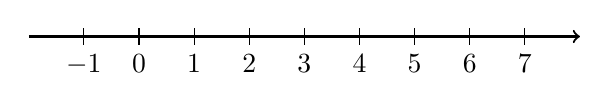
\begin{tikzpicture}[scale=0.7]
  \draw[thick,->] (-2,0) -- (8,0);
  \foreach \x in {-1,...,7} \draw (\x,0.15) -- (\x,-0.15) node[below] {$\x$};
\end{tikzpicture}
\end{center}
\end{questionText}
\correctAnswer{$x < 3$; open circle at $3$, shade left}
\explanation{Subtract $9$: $-3x > -9$. Divide by $-3$ and flip: $x < 3$. Open circle at $3$, shade left.}
\end{practiceQuestion}

\begin{practiceQuestion}{5-6-q30}{gsa}
\begin{questionText}
A student has test scores of $78$, $85$, and $90$. She needs an average of at least $85$ on four tests to earn an A. Solve the inequality to find the minimum score $s$ on the fourth test, and describe the graph.

\begin{center}
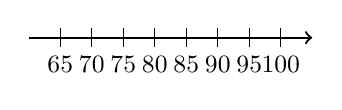
\begin{tikzpicture}[scale=0.08]
  \draw[thick,->] (60,0) -- (105,0);
  \foreach \x in {65,70,...,100} {
    \draw (\x,1.5) -- (\x,-1.5) node[below,font=\small] {$\x$};
  }
\end{tikzpicture}
\end{center}
\end{questionText}
\correctAnswer{$s \geq 87$; closed circle at $87$, shade right}
\explanation{$\frac{78 + 85 + 90 + s}{4} \geq 85$. Multiply by $4$: $253 + s \geq 340$. Subtract $253$: $s \geq 87$. Closed circle at $87$, shade right.}
\end{practiceQuestion}
